\section{Saalübung zu Energiewirtschaft}

\textbf{Beispiele für OR in der Energiewirtschaft:}
\begin{itemize}
	\item Netzplanung
	\item Minimierung der Umwandlungsverluste
	\item Maximierung der Erlöse aus der Strom- und Wärmeproduktion
	\item Minimierung der Betriebskosten
\end{itemize}
\bigskip
\textbf{Kosten der Stromerzeugung:}
\begin{center}
	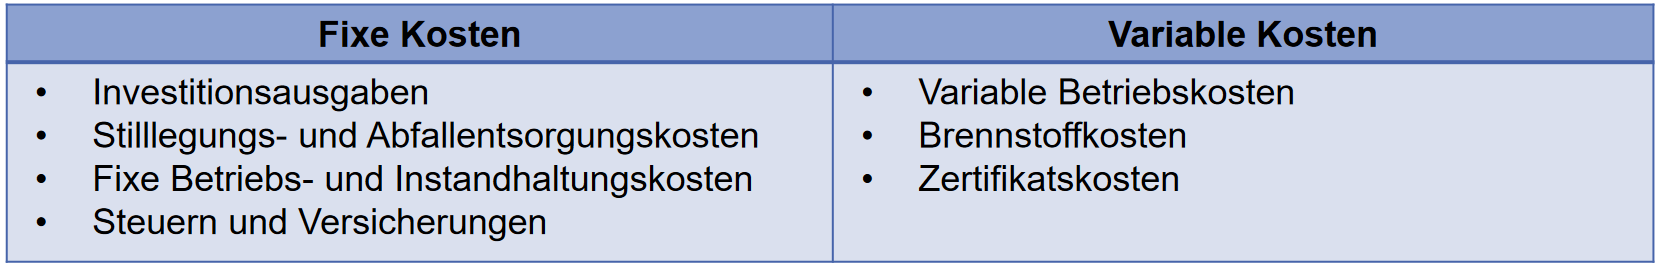
\includegraphics[width=0.8\textwidth]{images/costs.png}
\end{center}
\begin{itemize}
	\item Erzeugungstechnologien unterscheiden sich stark bei Kostenstruktur
	\item Vergleich der Kosten von Erzeugungstechnologien durch:
	\begin{itemize}
		\item Statische Kostenvergleichsrechnung: \textbf{Screening Kurven}
		\item Dynamische Investitionsrechnung: \textbf{Stromgestehungskosten (LCOE)}
	\end{itemize}
\end{itemize}
\bigskip
\textbf{Screening Kurven:}
\begin{itemize}
	\item Stellen Gesamtkosten/Durchschnittskosten einer Erzeugungstechnologie pro Jahr und pro Kapazitätseinheit dar
	\item Vergleich von Kostenstrukturen der verschiedenen Technologien
	
	$\rightarrow$ Bestimmung der kostengünstigsten Erzeugungstechnologie in Abhängigkeit der Volllaststunden
	
	\item \textbf{Gesamtkostenkurve}: $K_{ges}(t)=I_0\cdot a+ C^{var}\cdot t$ mit $I_0$: Kapitalkosten, $a$: Annuitätenfaktor, $C^{var}$: variable Kosten, $t$: Volllaststunden
	\item $a=\frac{(1+r)^T\cdot r}{(1+r)^T -1}$
	\begin{center}
		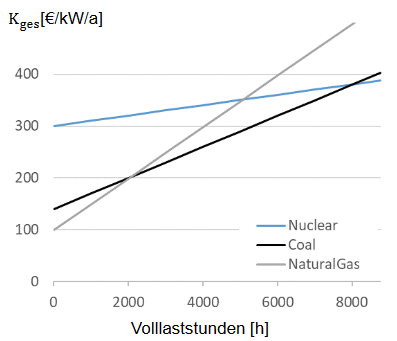
\includegraphics[width=0.4\textwidth]{images/gkk.png}
	\end{center}

	\item \textbf{Durchschnittskostenkurve}: Mit steigenden Volllaststunden nähern sich die
	Durchschnittskosten den variablen Kosten an
	\begin{center}
		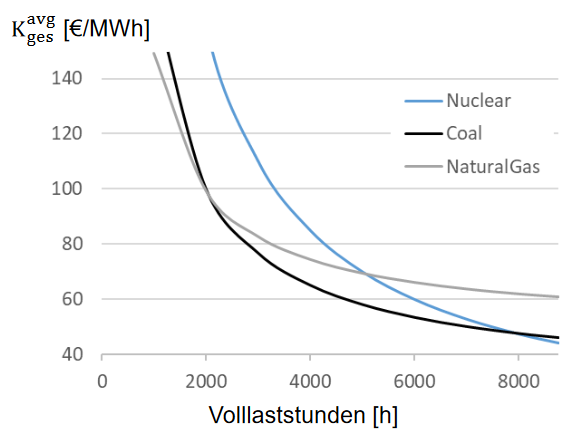
\includegraphics[width=0.4\textwidth]{images/dkk.png}
	\end{center}
\end{itemize}

\textbf{Stromgestehungskosten:}
\begin{itemize}
	\item Levelized costs of electricity (LCOE)
	\item Alle Kosten, die bei Umwandlung einer Energieform in elektrischen Strom anfallen
	\item \textbf{Kosten des Kraftwerkbetriebs}: Kosten für Errichtung und jährlichen Betrieb einer Anlage im Verhältnis zur Stromerzeugungsmenge der gesamte Lebensdauer
	\item \textbf{Nachteile}: Keine Aussage über Wirtschaftlichkeit der Anlage, Flexibilität der Anlage wird nicht berücksichtigt
	\begin{center}
		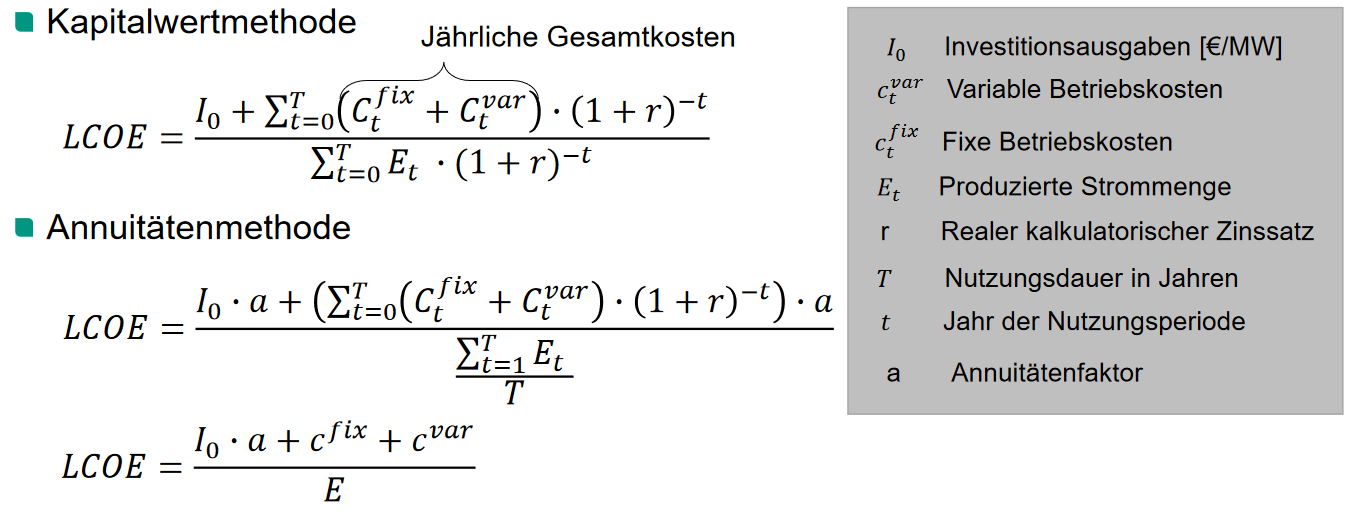
\includegraphics[width=0.7\textwidth]{images/sgk.png}
	\end{center}
	\item \textbf{Einheit}: \textit{\euro}$/MWh$ oder $Cent/kWh$
\end{itemize}
\textit{Beispielrechnung: Übung F25-26}\\

\textbf{Unit commitment model:} OR-Modell zur Kraftwerkseinsatzoptimierung
\begin{itemize}
	\item \textbf{Zielfunktion}: $
	\min\limits_{y_{u t}, s_{u t}} \sum\limits_{t=1}^{T} \sum\limits_{u} c_{u}^{v a r} \cdot y_{u t} \cdot \Delta t+\sum\limits_{t=1}^{T} \sum\limits_{u}\left(c_{u}^{\text {start }} \cdot s_{u t}\right)
	$
	\item \textbf{Nebenbedingungen}:
	\begin{enumerate}
		\item Gleichgewicht bei Nachfrage und Angebot: $\sum\limits_{u} y_{u t} \cdot \Delta t=D_{t} \cdot \Delta t \quad \forall t$
		\item Kapazitätsgrenzen der Technologien: $y_{u t} \leq K_{u} \cdot o_{u t} \quad \forall u, t$
		\item Minimale Produktionsgrenze: $y_{u t} \geq P_{u}^{\min } \cdot o_{u t} \quad \forall u, t$
		\item Start-up Bedingungen: $s_{u t} \geq o_{u t}-o_{u, t-1} \quad \forall u, t$
		\item Erzeugung durch Erneuerbare Energien: $y_{u t} \leq w_{u t} \cdot K_{u} \quad \forall u, t$
		\item Variablenschranken: $$
		\begin{array}{ll}
			y_{u t}, D_{t} \geq 0 & \forall u, t \\
			o_{u t}, s_{u t} \text { Binärvariable } & \forall u, t
		\end{array}
		$$
	\end{enumerate}
	\item \textbf{Variablen}:\qquad
	$\begin{array}{ll}u \in U & \text { Erzeugungstechnologien } \\ c_{u}^{v a r} & \text { Variable Kosten } \\ y_{u t} & \text { Output } \\ \Delta t & \text { Zeitschritt } \\ c_{u}^{\text {start }} & \text { Kosten für start-ups } \\ s_{u t} & \text { Entscheidungsvariable für start-ups } \\ o_{u t} & \text { Entscheidungsvariable für Betrieb } \\ D_{t} & \text { Nachfrage } \\ K_{u} & \text { Installierte Kapazität } \\ P_{u}^{\text {min }} & \text { Min. Outputlevel }\end{array}$
\end{itemize}
\bigskip
\textbf{OR-Modell: Investitionsplanung und Kraftwerkseinsatz:}
\begin{center}
	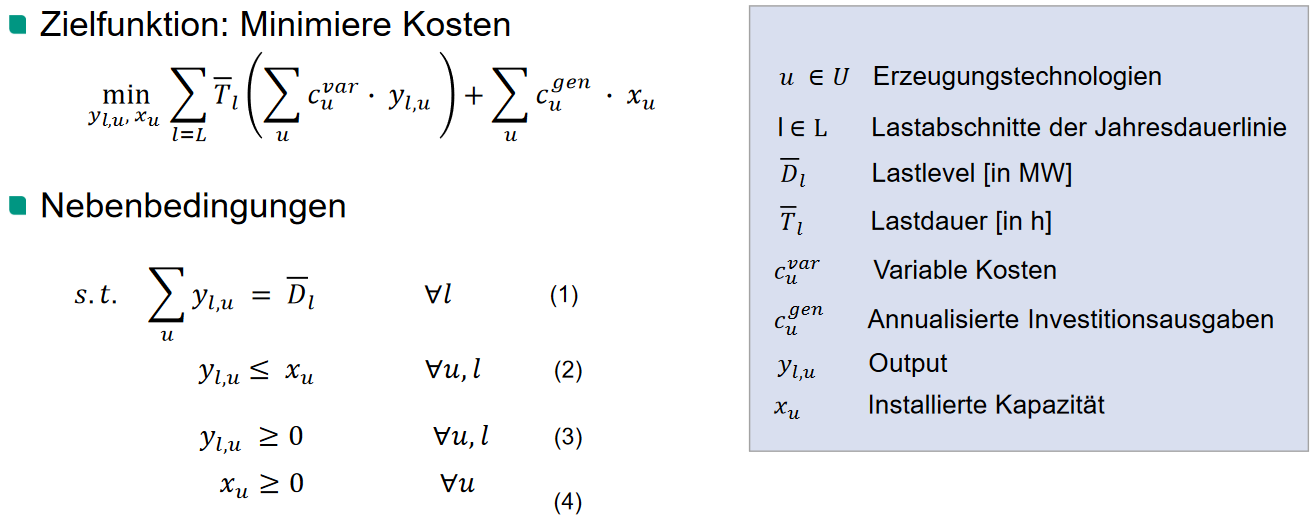
\includegraphics[width=0.8\textwidth]{images/or.png}
\end{center}